
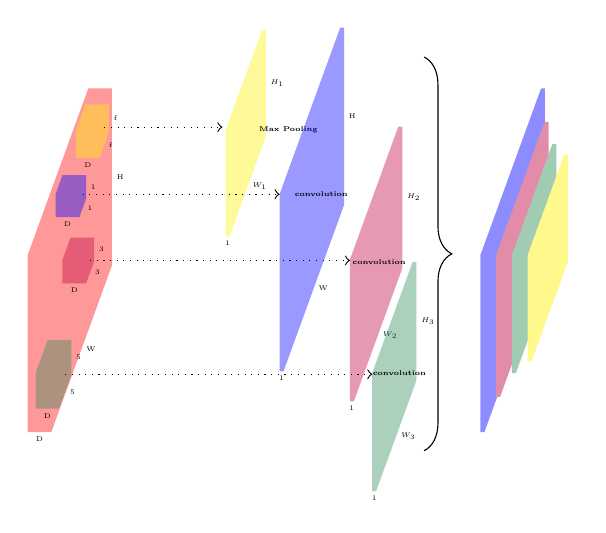
\begin{tikzpicture}[scale=0.5,transform shape]
	
	\pgfsetxvec{\pgfpoint{1cm}{0cm}}
	\pgfsetyvec{\pgfpoint{0cm}{1cm}}
	\pgfsetzvec{\pgfpoint{-.342cm}{-.94cm}}
	
	\def\cuboid#1#2#3#4#5{
	\begin{scope}
	\edef\mycolor{#2}
	\edef\depth{#3}
	\edef\height{#4}
	\edef\width{#5}
	\draw[black,fill=\mycolor, fill opacity=0.4, text opacity=1] #1 -- ++(-\depth,0,0) -- ++(0,-\height,0) -- ++(\depth,0,0) -- cycle #1 -- ++(0,0,-\width) -- ++(0,-\height,0) -- ++(0,0,\width) -- cycle  #1 -- ++(-\depth,0,0) -- ++(0,0,-\width) -- ++(\depth,0,0) -- cycle;
	\end{scope}
	}
	
	\def\cuboidlabel#1#2#3#4#5#6#7#8{
	\begin{scope}
	\edef\mycolor{#2}
	\edef\depth{#3}
	\edef\height{#4}
	\edef\width{#5}
	\edef\depthlabel{#6}
	\edef\heightlabel{#7}
	\edef\widthlabel{#8}
	\draw[draw=none,fill=\mycolor, fill opacity=0.4, text opacity=1] #1 -- ++(-\depth,0,0) -- ++(0,-\height,0) -- ++(\depth,0,0) node[pos=0.5,below] {\tiny \depthlabel} -- cycle #1 -- ++(0,0,-\width) -- ++(0,-\height,0) node[pos=0.5,right] {\tiny \heightlabel} -- ++(0,0,\width)  node[pos=0.5,below,right] {\tiny \widthlabel} -- cycle  #1 -- ++(-\depth,0,0) -- ++(0,0,-\width) -- ++(\depth,0,0) -- cycle;
	\end{scope}
	}
	
	\def\kernel#1#2#3#4#5#6{
	\begin{scope}
	\edef\mycolor{#2}
	\edef\depth{#3}
	\edef\height{#4}
	\edef\width{#5}
	\draw[black,fill=\mycolor, fill opacity=0.4, text opacity=1] #1 -- ++(-\depth,0,0) -- ++(0,-\height,0) -- ++(\depth,0,0) -- cycle #1 -- ++(0,0,-\width) -- ++(0,-\height,0) -- ++(0,0,\width) -- cycle  #1 -- ++(-\depth,0,0) -- ++(0,0,-\width) -- ++(\depth,0,0) -- cycle;
	
	\draw[dotted] #1 -- #6 #1++(0,0,-\width) -- #6 #1++(0,-\height,0) -- #6 #1++(0,-\height,-\width) -- #6;
	
	\end{scope}
	}
	
	\def\kernellabel#1#2#3#4#5#6#7#8#9{
	%#6 is target pixel
	\begin{scope}
	\edef\mycolor{#2}
	\edef\depth{#3}
	\edef\height{#4}
	\edef\width{#5}
	\edef\depthlabel{#7}
	\edef\heightlabel{#8}
	\edef\widthlabel{#9}
	\draw[draw=none,fill=\mycolor, fill opacity=0.4, text opacity=1] #1 -- ++(-\depth,0,0) -- ++(0,-\height,0) -- ++(\depth,0,0) node[pos=0.5,below] {\tiny \depthlabel} -- cycle #1 -- ++(0,0,-\width) -- ++(0,-\height,0) node[pos=0.5,right] {\tiny \heightlabel} -- ++(0,0,\width)  node[pos=0.5,below,right] {\tiny \widthlabel} -- cycle  #1 -- ++(-\depth,0,0) -- ++(0,0,-\width) -- ++(\depth,0,0) -- cycle;
	\end{scope}
	}
	
	\def\kernellabell#1#2#3#4#5#6#7#8#9{
	%#6 is target pixel
	\begin{scope}
	\edef\mycolor{#2}
	\edef\depth{#3}
	\edef\height{#4}
	\edef\width{#5}
	\edef\depthlabel{#7}
	\edef\heightlabel{#8}
	\edef\widthlabel{#9}
	\draw[draw=none,fill=\mycolor,  text opacity=1] #1 -- ++(-\depth,0,0) -- ++(0,-\height,0) -- ++(\depth,0,0) node[pos=0.5,below] {} -- cycle #1 -- ++(0,0,-\width) -- ++(0,-\height,0) node[pos=0.5,right] {} -- ++(0,0,\width)  node[pos=0.5,below,right] {} -- cycle  #1 -- ++(-\depth,0,0) -- ++(0,0,-\width) -- ++(\depth,0,0) -- cycle;
	
	%\draw[->] #10 -- #6 ;%#1++(0,0,-\width) -- #6 #1++(0,-\height,0) -- #6 #1++(0,-\height,-\width) -- #6;
	\end{scope}
	}
	
	
	%alexnet
	\onslide<1->{
	\cuboidlabel{(2,-0.5,-0.5)}{red}{0.6}{4.5}{4.5}{D}{H}{W}
	}
	
	\onslide<2->{
	\kernellabel{(2.2,-0.15,-3.5)}{yellow}{0.6}{0.7}{0.7}{(3.7,-2.5,-2.5)}{D}{f}{f}
	\draw [dotted,->] (2.2, -0.4,-3.85) -- (5.2, -0.4, -3.85);
	\kernellabel{(5.5,-0.15,-3.5)}{yellow}{0.1}{2.7}{2.7}{(3.7,-2.5,-2.5)}{1}{$H_1$}{$W_1$}
	\node (T) at (7,-0.15,-3.5){\textbf{\tiny{Max Pooling}}};
	
	}
	
	\onslide<3->{
	\kernellabel{(2.2,-0.35,-2)}{blue}{0.6}{0.6}{0.5}{(3.7,-2.5,-2.5)}{D}{1}{1}
	\draw [dotted,->] (2.2, -0.6,-2.25) -- (7.2, -0.6, -2.25);
	\kernellabel{(7.3,-0.6,-2.25)}{blue}{0.1}{4.5}{4.5}{(3.7,-2.5,-2.5)}{1}{H}{W}
	\node (T) at (8.3,-0.35,-2){\textbf{\tiny{\text{ convolution}}}};
	}
	
	\onslide<4->{
	\kernellabel{(2.2,-2.5,-2.5)}{purple}{0.6}{0.6}{0.6}{(3.7,-2.5,-2.5)}{D}{3}{3}
	\draw [dotted,->] (2.2,-2.8,-2.8) -- (8.8,-2.8,-2.8);
	\kernellabel{(9,-2.5,-2.5)}{purple}{0.1}{3.6}{3.6}{(3.7,-2.5,-2.5)}{1}{$H_2$}{$W_2$}
	\node (T) at (9.6,-2.55,-2.5){\textbf{\tiny{\text{ convolution}}}};
	}
	
	\onslide<5->{
	\kernellabel{(2.2,-3.5,-0.5)}{SeaGreen}{0.6}{0.9}{0.9}{(3.7,-2.5,-2.5)}{D}{5}{5}
	\draw [dotted,->] (2.2,-3.95,-0.95) -- (10,-3.95,-0.95);
	\kernellabel{(10.25,-3.5,-0.5)}{SeaGreen}{0.1}{3}{3}{(3.7,-2.5,-2.5)}{1}{$H_3$}{$W_3$}
	\node (T) at (10.8,-3.5,-0.5){\textbf{\tiny{\text{ convolution}}}};
	}
	
	
	\onslide<7->{
	\draw [decorate,decoration={brace,amplitude=10pt, mirror},xshift=4pt,yshift=0pt]
	(11.5,-5,0) -- (11.5, 5,0) node [black,midway,xshift=0.6cm] 
	{};
	}
	\onslide<7->{
	\kernellabell{(13,-0.5,-0.5)}{blue!45!white}{0.1}{4.5}{4.5}{(3.7,-2.5,-2.5)}{D}{5}{5}
	\kernellabell{(13.4,-0.5,-0.5)}{purple!45!white}{0.1}{3.6}{3.6}{(3.7,-2.5,-2.5)}{D}{5}{5}
	\kernellabell{(13.8,-0.5,-0.5)}{SeaGreen!45!white}{0.1}{3}{3}{(3.7,-2.5,-2.5)}{D}{5}{5}
	\kernellabell{(14.2,-0.5,-0.5)}{yellow!45!white}{0.1}{2.7}{2.7}{(3.7,-2.5,-2.5)}{1}{5}{5}

}
\end{tikzpicture}
